              %******************************************%
              %                                          %
              % Modello di tesi di laurea o di dottorato %
              %            di Lorenzo Pantieri ©         %
              %                                          %
              %         versione: 14 aprile 2013         %
              %                                          %
              %******************************************%
       

% I seguenti commenti speciali impostano:
% 1. utf8 come codifica di input,
% 2. PDFLaTeX come motore di composizione;
% 3. Tesi.tex come documento principale;
% 4. il controllo ortografico italiano per l'editor.

% !TEX encoding = UTF-8 Unicode
% !TEX TS-program = pdflatex
% !TEX root = Tesi.tex
% !TEX spellcheck = it-IT

\documentclass[10pt,%                      % corpo del font principale
               a4paper,%                   % carta A4
               twoside,openright,%         % fronte-retro
%              oneside,openany,%           % solo fronte
               titlepage,%                 % frontespizio
               headinclude,,footinclude,%  % testatina e piede di pagina
               BCOR5mm,%                   % rilegatura di 5 mm
               cleardoublepage=empty,%     % pagine vuote senza testatina e piede di pagina
               tablecaptionabove,%         % didascalie in cima alle tabelle
               ]{scrreprt}                 % classe report di KOMA-Script;
               
\usepackage[T1]{fontenc}                   % codifica dei font:
                                           % NOTA BENE! richiede una distribuzione *completa* di LaTeX,
                                           % per esempio TeXLive o MiKTeX *complete*

\usepackage[utf8]{inputenc}                % codifica di input; anche [latin1] va bene
                                           % NOTA BENE! va accordata con le preferenze dell'editor

\usepackage[english,italian]{babel}        % per scrivere in italiano e in inglese;
                                           % l'ultima lingua (l'italiano) risulta predefinita

\usepackage[suftesi]{frontespizio}         % frontespizo
                                           % per includerlo nel documento bisogna:
                                           % 1. compilare una prima volta Tesi.tex;
                                           % 2. compilare a parte Tesi-frn.tex, generato dalla compilazione precedente;
                                           % 3. compilare ancora Tesi.tex. 

\usepackage{indentfirst}                   % rientra il primo capoverso di ogni sezione

\usepackage{graphicx}                      % immagini

\usepackage{listings}                      % codici

\usepackage[font=small]{quoting}           % citazioni

\usepackage{amsmath,amssymb,amsthm}        % matematica

\usepackage[italian]{varioref}             % riferimenti completi della pagina

\usepackage{mparhack,fixltx2e,relsize}     % finezze tipografiche

\usepackage{tabularx}                      % tabelle di larghezza prefissata

\usepackage[style=philosophy-modern,hyperref,backref,square,natbib,backend=biber]{biblatex}
                                           % eccellente pacchetto per la bibliografia;
                                           % produce uno stile di citazione autore-anno; 
                                           % lo stile "numeric-comp" produce riferimenti numerici;
                                           % NOTA BENE! bisogna che il proprio editor sia configurato per biber
                                          
\addbibresource{Bibliografia.bib}          % database di biblatex 
                                          
\usepackage{subfig}                        % sottofigure, sottotabelle

\usepackage{lipsum}                        % testo fittizio

\usepackage{eurosym}                       % simbolo dell'euro

\usepackage[eulerchapternumbers,%          % numeri dei capitoli nel font Euler
            subfig,%                       % se si usa il pacchetto subfig
            beramono,%                     % Bera Mono come font a spaziatura fissa
            eulermath,%                    % AMS Euler come font per la matematica
            pdfspacing,%                   % migliora il riempimento di riga
            listings,%                     % codici
%           parts,%                        % da decommentare in un documento diviso in parti
            ]{classicthesis}               % stile ClassicThesis

\usepackage{arsclassica}                   % modifica alcuni aspetti di ClassicThesis

\usepackage{bookmark}                      % segnalibri

%*********************************************************************************
% impostazioni-tesi.tex
% di Lorenzo Pantieri (2011-2013)
% file che contiene le impostazioni della tesi
%*********************************************************************************


%*********************************************************************************
% Comandi personali
%*******************************************************
\newcommand{\myName}{Lorenzo Pantieri}                       % autore
\newcommand{\myTitle}{La prova ontologica dell'esistenza di Dio} % titolo
\newcommand{\myDegree}{Tesi di laurea}                       % tipo di tesi
\newcommand{\myUni}{Universit� degli Studi del Magdeburgo} % universit�
\newcommand{\myFaculty}{Facolt� di Lettere e Filosofia}    % facolt�
\newcommand{\myDepartment}{Dipartimento di Teologia}         % dipartimento
\newcommand{\myProf}{Chiar.mo Prof.~S.~Anselmo d'Aosta}      % relatore
%\newcommand{\myOtherProf}{Dott.~Immanuel Kant}              % correlatore (se c'�)
\newcommand{\myLocation}{Magdeburgo}                         % dove
\newcommand{\myTime}{Aprile 2013}                          % quando



%*********************************************************************************
% Impostazioni di amsmath, amssymb, amsthm
%*********************************************************************************

% comandi per gli insiemi numerici (serve il pacchetto amssymb)
\newcommand{\numberset}{\mathbb} 
\newcommand{\N}{\numberset{N}} 
\newcommand{\R}{\numberset{R}} 

% un ambiente per i sistemi
\newenvironment{sistema}%
  {\left\lbrace\begin{array}{@{}l@{}}}%
  {\end{array}\right.}

% definizioni (serve il pacchetto amsthm)
\theoremstyle{definition} 
\newtheorem{definizione}{Definizione}

% teoremi, leggi e decreti (serve il pacchetto amsthm)
\theoremstyle{plain} 
\newtheorem{teorema}{Teorema}
\newtheorem{legge}{Legge}
\newtheorem{decreto}[legge]{Decreto}
\newtheorem{murphy}{Murphy}[section]



%*********************************************************************************
% Impostazioni di biblatex
%*********************************************************************************
\defbibheading{bibliography}{%
\cleardoublepage
\manualmark
\phantomsection 
\addcontentsline{toc}{chapter}{\tocEntry{\bibname}}
\chapter*{\bibname\markboth{\spacedlowsmallcaps{\bibname}}
{\spacedlowsmallcaps{\bibname}}}}



%*********************************************************************************
% Impostazioni di listings
%*********************************************************************************
\lstset{language=[LaTeX]Tex,%C++,
    keywordstyle=\color{RoyalBlue},%\bfseries,
    basicstyle=\small\ttfamily,
    %identifierstyle=\color{NavyBlue},
    commentstyle=\color{Green}\ttfamily,
    stringstyle=\rmfamily,
    numbers=none,%left,%
    numberstyle=\scriptsize,%\tiny
    stepnumber=5,
    numbersep=8pt,
    showstringspaces=false,
    breaklines=true,
    frameround=ftff,
    frame=single
} 



%*********************************************************************************
% Impostazioni di hyperref
%*********************************************************************************
\hypersetup{%
    hyperfootnotes=false,pdfpagelabels,
    %draft,	% = elimina tutti i link (utile per stampe in bianco e nero)
    colorlinks=true, linktocpage=true, pdfstartpage=1, pdfstartview=FitV,%
    % decommenta la riga seguente per avere link in nero (per esempio per la stampa in bianco e nero)
    %colorlinks=false, linktocpage=false, pdfborder={0 0 0}, pdfstartpage=1, pdfstartview=FitV,% 
    breaklinks=true, pdfpagemode=UseNone, pageanchor=true, pdfpagemode=UseOutlines,%
    plainpages=false, bookmarksnumbered, bookmarksopen=true, bookmarksopenlevel=1,%
    hypertexnames=true, pdfhighlight=/O,%nesting=true,%frenchlinks,%
    urlcolor=webbrown, linkcolor=RoyalBlue, citecolor=webgreen, %pagecolor=RoyalBlue,%
    %urlcolor=Black, linkcolor=Black, citecolor=Black, %pagecolor=Black,%
    pdftitle={\myTitle},%
    pdfauthor={\textcopyright\ \myName, \myUni, \myFaculty},%
    pdfsubject={},%
    pdfkeywords={},%
    pdfcreator={pdfLaTeX},%
    pdfproducer={LaTeX with hyperref and ClassicThesis}%
}



%*********************************************************************************
% Impostazioni di graphicx
%*********************************************************************************
\graphicspath{{Immagini/}} % cartella dove sono riposte le immagini



%*********************************************************************************
% Margini ottimizzati per l'A4
%*********************************************************************************
\areaset[current]{336pt}{750pt}
\setlength{\marginparwidth}{7em}
\setlength{\marginparsep}{2em}%



%*********************************************************************************
% Impostazioni di varioref
%*********************************************************************************
\makeatletter
\vref@addto\extrasitalian{%
   \def\reftextfaraway#1{a pagina~\pageref{#1}}%
}
\makeatother



%*********************************************************************************
% Altro
%*********************************************************************************

% [...] ;-)
\newcommand{\omissis}{[\dots\negthinspace]}

% eccezioni all'algoritmo di sillabazione
\hyphenation{Fortran ma-cro-istru-zio-ne nitro-idrossil-amminico}

% correzione di un bug di scrreprt nella numerazione delle figure
\renewcommand*{\figureformat}{%
  \figurename~\thefigure%
  %\autodot%
}
\renewcommand*{\tableformat}{%
  \tablename~\thetable%
  %\autodot%
}


                  % file con le impostazioni personali


\begin{document}
\pagestyle{scrheadings} 
\pagenumbering{roman}
%******************************************************************
% Materiale iniziale
%******************************************************************
% !TEX encoding = UTF-8
% !TEX TS-program = pdflatex
% !TEX root = ../Tesi.tex
% !TEX spellcheck = it-IT

%*******************************************************
% Frontespizio
%*******************************************************
\begin{frontespizio}
\Preambolo{\usepackage{iwona}} % riga da commentare se non si carica ArsClassica

\Universita{Bologna}
\Logo{Sigillo}
\Facolta{Teologia}
\Corso{Belle Lettere}
\Annoaccademico{2012--2013}
\Titoletto{Tesi di laurea magistrale}
\Titolo{La mia tesi: \\ la prova ontologica \\ dell'esistenza di Dio}
\Sottotitolo{Alcune considerazioni mutevoli}
\Candidato[AB123456]{Lorenzo Pantieri}
\Relatore{Enrico Gregorio}
\Relatore{Claudio Beccari}
\Correlatore{Tommaso Gordini}
\Correlatore{Ivan Valbusa}
\end{frontespizio}





%*******************************************************
% Frontespizio alternativo
%*******************************************************
%\begin{titlepage}
%\pdfbookmark{Frontespizio}{Frontespizio}
%\changetext{}{}{}{((\paperwidth - \textwidth) / 2) - \oddsidemargin - \hoffset - 1in}{}
%\null\vfill
%\begin{center}
%\large
%\sffamily
%\bigskip

%{\LARGE\myName} \\

%\bigskip

%{\Huge\myTitle \\
%}

%\bigskip
    
%\vspace{9cm}

%\begin{tabular}{cc}
%\parbox{0.3\textwidth}{\includegraphics[width=2.5cm]{Sigillo}}
%&
%\parbox{0.7\textwidth}{{\Large\myDegree} \\ 

%					{\normalsize
%					Relatore: \myProf \\
%%					Co-relatore: \myOtherProf \\
%					
%					\myUni \\
%					\myFaculty \\
%					\myDepartment \\
%					\myTime}}
%			\end{tabular}
%\end{center}
%\vfill
%\end{titlepage}







% !TEX encoding = UTF-8
% !TEX TS-program = pdflatex
% !TEX root = ../Tesi.tex
% !TEX spellcheck = it-IT

%*******************************************************
% Colophon
%*******************************************************
\clearpage
\phantomsection
\thispagestyle{empty}

\hfill

\vfill

%\noindent\myName: \textit{\myTitle,}
%\myDegree,
%\textcopyright\ \MakeTextLowercase{\myTime}.

\lipsum[2]
% !TEX encoding = UTF-8
% !TEX TS-program = pdflatex
% !TEX root = ../Tesi.tex
% !TEX spellcheck = it-IT

%*******************************************************
% Dedica
%*******************************************************
\cleardoublepage
\phantomsection
\thispagestyle{empty}
\pdfbookmark{Dedica}{Dedica}

\vspace*{3cm}

\begin{center}
Lorem ipsum dolor sit amet, consectetuer adipiscing elit. \\ \medskip
--- Oscar Wilde    
\end{center}

\medskip

\begin{center}
Dedicato a tutti gli appassionati di \LaTeX.
\end{center}
% !TEX encoding = UTF-8
% !TEX TS-program = pdflatex
% !TEX root = ../Tesi.tex
% !TEX spellcheck = it-IT

%*******************************************************
% Indici
%*******************************************************
\cleardoublepage
\pdfbookmark{\contentsname}{tableofcontents}
\setcounter{tocdepth}{2}
\tableofcontents
\markboth{\spacedlowsmallcaps{\contentsname}}{\spacedlowsmallcaps{\contentsname}} 
\clearpage

\begingroup 
    \let\clearpage\relax
    \let\cleardoublepage\relax
    \let\cleardoublepage\relax
    %*******************************************************
    % Elenco delle figure
    %*******************************************************    
    \phantomsection
    \pdfbookmark{\listfigurename}{lof}
    \listoffigures

    \vspace*{8ex}

    %*******************************************************
    % Elenco delle tabelle
    %*******************************************************
    \phantomsection
    \pdfbookmark{\listtablename}{lot}
    \listoftables
        
    \vspace*{8ex}
       
\endgroup

\cleardoublepage

% !TEX encoding = UTF-8
% !TEX TS-program = pdflatex
% !TEX root = ../Tesi.tex
% !TEX spellcheck = it-IT

%*******************************************************
% Sommario+Abstract
%*******************************************************
\cleardoublepage
\phantomsection
\pdfbookmark{Sommario}{Sommario}
\begingroup
\let\clearpage\relax
\let\cleardoublepage\relax
\let\cleardoublepage\relax

\chapter*{Sommario}

\lipsum[1]

\vfill

\selectlanguage{english}
\pdfbookmark{Abstract}{Abstract}
\chapter*{Abstract}

\lipsum[2]

\selectlanguage{italian}

\endgroup			

\vfill


% !TEX encoding = UTF-8
% !TEX TS-program = pdflatex
% !TEX root = ../Tesi.tex
% !TEX spellcheck = it-IT

%*******************************************************
% Ringraziamenti
%*******************************************************
\cleardoublepage
\phantomsection
\pdfbookmark{Ringraziamenti}{ringraziamenti}

\begin{flushright}{\slshape    
	Lorem ipsum dolor sit amet, consectetuer adipiscing elit. \\
	Ut purus elit, vestibulum ut, placerat ac, adipiscing vitae, felis. \\
	Curabitur dictum gravida mauris.} \\ \medskip
    --- Donald Ervin Knuth
\end{flushright}


\bigskip

\begingroup
\let\clearpage\relax
\let\cleardoublepage\relax
\let\cleardoublepage\relax

\chapter*{Ringraziamenti}

\lipsum[1]

\bigskip
 
\noindent\textit{\myLocation, \MakeTextLowercase{\myTime}}
\hfill L.~P.

\endgroup
% !TEX encoding = UTF-8
% !TEX TS-program = pdflatex
% !TEX root = ../Tesi.tex
% !TEX spellcheck = it-IT

%*******************************************************
% Introduzione
%*******************************************************
\cleardoublepage
\pdfbookmark{Introduzione}{introduzione}

\chapter*{Introduzione}

\lipsum[1]

Lorem ipsum dolor sit amet, consectetuer adipiscing elit.
\begin{description}
\item[{\hyperref[cap:lorem]{Il primo capitolo}}]
offre una visione d'insieme della storia di \LaTeX{} e ne vengono presentate le idee di fondo.
\item[{\hyperref[cap:ipsum]{Il secondo capitolo}}]
spiega le operazioni, veramente semplici, per installare \LaTeX{} sul proprio calcolatore.
\item[{\hyperref[cap:dolor]{L'appendice A}}] descrive  sinteticamente le principali norme tipografiche della lingua italiana, utili nella composizione di articoli, tesi o libri.
\end{description}

\lipsum[2]
\cleardoublepage
%******************************************************************
% Materiale principale
%******************************************************************
\pagenumbering{arabic}
% !TEX encoding = UTF-8
% !TEX TS-program = pdflatex
% !TEX root = ../Tesi.tex
% !TEX spellcheck = it-IT

%************************************************
\chapter{Lorem}
\label{cap:lorem}
%************************************************

Lorem ipsum dolor sit amet, consectetuer adipiscing elit. Ut purus elit, vestibulum ut, placerat ac, adipiscing vitae, felis. Curabitur dictum gravida mauris. Nam arcu libero, nonummy eget, consectetuer id, vulputate a, magna. Donec vehicula augue eu neque.

\section{Esempi}

\subsection{Tabelle}

\lipsum

\begin{table}[tb]
\caption[Un esempio di tabella mobile]{Un esempio di tabella mobile.}
\label{tab:esempio}
\centering
\begin{tabular}{cc}
\toprule
$p$ & $\lnot p$ \\ 
\midrule
V   & F \\ 
F   & V \\
\bottomrule 
\end{tabular}
\end{table}

La tabella~\vref{tab:esempio} fornisce un esempio di tabella mobile.

\lipsum[1-2]


\subsection{Figure}

\lipsum[2]

\begin{figure}[tb] 
\centering 
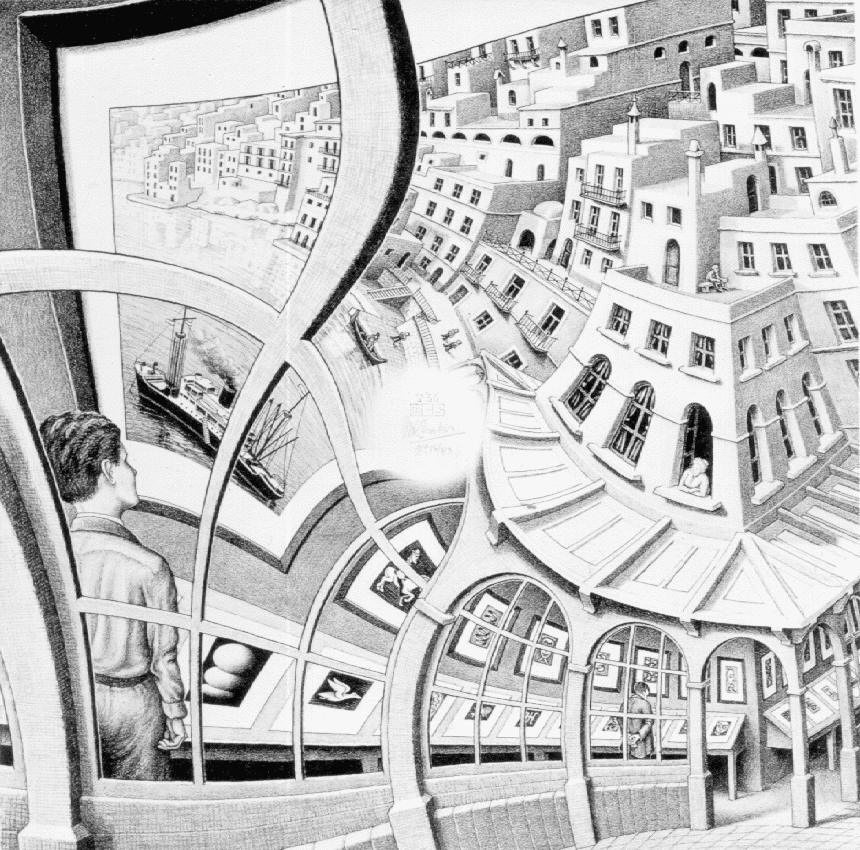
\includegraphics[width=0.5\columnwidth]{GalleriaStampe} 
\caption[Un esempio di figura mobile]{Un esempio di figura mobile (l'immagine, che riproduce la litografia \emph{Galleria di stampe}, di M.~Escher,\index{Escher, M.~C.} proviene da \url{http://www.mcescher.com/}).}
\label{fig:galleria} 
\end{figure}

La figura~\vref{fig:galleria} fornisce un esempio di figura mobile.

\lipsum[3]

\begin{figure}[tb]
\centering
\subfloat[Asia personas duo.]
{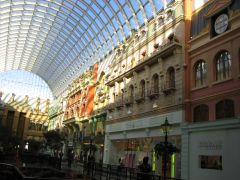
\includegraphics[width=.45\columnwidth]{Lorem}} \quad
\subfloat[Pan ma signo.]
{\label{fig:ipsum}%
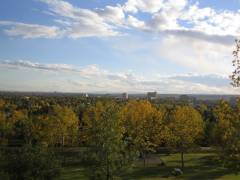
\includegraphics[width=.45\columnwidth]{Ipsum}} \\
\subfloat[Methodicamente o uno.]
{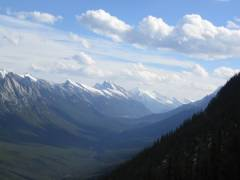
\includegraphics[width=.45\columnwidth]{Dolor}} \quad
\subfloat[Titulo debitas.]
{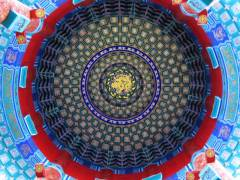
\includegraphics[width=.45\columnwidth]{Sit}}
\caption[Tu duo titulo debitas latente]{Tu duo titulo debitas
latente.}
\label{fig:esempio}
\end{figure}

La figura~\vref{fig:esempio} costituisce un esempio di figura mobile.

\lipsum[4]

% !TEX encoding = UTF-8
% !TEX TS-program = pdflatex
% !TEX root = ../Tesi.tex
% !TEX spellcheck = it-IT

%************************************************
\chapter{Ipsum}
\label{cap:ipsum}
%************************************************


Lorem ipsum dolor sit amet, consectetuer adipiscing elit. Nam dui ligula, fringilla a, euismod sodales, sollicitudin vel, wisi. Morbi auctor lorem non justo. Nam lacus libero, pretium at, lobortis vitae, ultricies et, tellus.
\begin{description}
\item[Lorem ipsum dolor] sit amet, consectetuer adipiscing elit. Ut purus elit, vestibulum ut, placerat ac $\lim_{n \to \infty}\sum_{k=1}^n \frac{1}{k^2}= \frac{\pi^2}{6}$.
\item[Mauris ut leo.]
Cras viverra metus rhoncus sem. Nulla et lectus vestibulum urna fringilla ultrices. Phasellus eu tellus sit amet tortor gravida placerat.
\[
\lim_{n \to \infty}\sum_{k=1}^n \frac{1}{k^2}= \frac{\pi^2}{6}.
\]
\end{description}

Nulla malesuada porttitor diam. Donec felis erat, congue non, volutpat at, tincidunt tristique, libero. Vivamus viverra fermentum felis.
\begin{equation}
\label{eq:euler}
e^{i\pi}+1=0.
\end{equation}
Dalla formula~\eqref{eq:euler} 
si deduce che\dots






\section{Nozioni basilari}

\subsection{Insiemi numerici}

Donec nonummy pellentesque ante. Phasellus adipiscing semper elit.
\begin{equation}
x^2 \geq 0 \quad
\forall x \in \mathbb{R}.
\end{equation}


\subsection{Le matrici}

\lipsum[2]
\begin{equation}
A=
\begin{bmatrix}
x_{11} & x_{12} & \dots \\
x_{21} & x_{22} & \dots \\
\vdots & \vdots & \ddots
\end{bmatrix}
\end{equation}



\section{Formule fuori corpo}

Proin fermentum massa ac quam. Sed diam turpis, molestie vitae, placerat a, molestie nec, leo. Maecenas lacinia. Nam ipsum ligula, eleifend at, accumsan nec, suscipit a, ipsum. 


\subsection{Una formula spezzata con allineamento}

\lipsum[2]
\begin{equation} 
\begin{split} 
a &= b+c-d \\ 
  &= e-f \\ 
  &= g+h \\ 
  &= i. 
\end{split} 
\end{equation}

 
\subsection{Casi}

\lipsum[3]
\begin{equation}
f(n):=
\begin{cases} 
2n+1, & \text{con $n$ dispari,} \\ 
n/2,  & \text{con $n$ pari.} 
\end{cases} 
\end{equation}



\section{Enunciati e dimostrazioni}

Nunc eleifend consequat lorem. Sed lacinia nulla vitae enim. Pellentesque tincidunt purus vel magna. Integer non enim. Praesent euismod nunc eu purus.
\begin{definizione}[di Gauss] 
Un \emph{matematico} trova ovvio che
$\int_{-\infty}^{+\infty}
e^{-x^2}\,dx=\sqrt{\pi}$. 
\end{definizione} 
\begin{teorema} 
I matematici, se ce ne sono, sono molto rari.
\end{teorema} 

\lipsum[2]

\begin{teorema}[di Pitagora]
La somma dei quadrati costruiti sui cateti uguaglia il quadrato costruito sull'ipotenusa.
\end{teorema}
La dimostrazione viene lasciata per esercizio.

Donec bibendum quam in tellus. Nullam cursus pulvinar lectus. Donec et mi. Nam vulputate metus eu enim. Vestibulum pellentesque felis eu massa.
\begin{teorema}[Sorpresa]
Si ha che $\log(-1)^2=2\log(-1)$.
\end{teorema} 
\begin{proof} 
Si ha che $\log(1)^2 = 2\log(1)$.
Ma si ha anche che $\log(-1)^2=\log(1)=0$.
Quindi $2\log(-1)=0$, da cui la tesi.
\end{proof}
Viene un quadratino a fine dimostrazione.
\begin{legge}
\label{lex:capo}
Il capo ha ragione.
\end{legge}
\begin{decreto}[Aggiornamento alla legge~\ref{lex:capo}]
Il capo ha \emph{sempre} ragione.
\end{decreto}
\begin{legge}
Se il capo ha torto, vedere la 
legge~\ref{lex:capo}.
\end{legge}


Nam dui ligula, fringilla a, euismod sodales, sollicitudin vel, wisi. Morbi auctor lorem non justo. Nam lacus libero, pretium at, lobortis vitae, ultricies et, tellus.
\begin{murphy}
Cras nec ante. Pellentesque a nulla. Cum sociis natoque penatibus et magnis dis parturient montes, nascetur ridiculus mus. Aliquam tincidunt urna.
\end{murphy}

\appendix
% !TEX encoding = UTF-8
% !TEX TS-program = pdflatex
% !TEX root = ../Tesi.tex
% !TEX spellcheck = it-IT

%************************************************
\chapter{Dolor}
\label{cap:dolor}
%************************************************

\lipsum[1]

\section{Mane}
\lipsum[2]

\section{Tekel}
\lipsum[3]

\section{Fares}
\lipsum[4-5]

% *****************************************************************
% Materiale finale
%******************************************************************
% !TEX encoding = UTF-8
% !TEX TS-program = pdflatex
% !TEX root = ../Tesi.tex
% !TEX spellcheck = it-IT

%*******************************************************
% Bibliografia
%*******************************************************
\cleardoublepage
\nocite{*}
\printbibliography
% !TEX encoding = UTF-8
% !TEX TS-program = pdflatex
% !TEX root = ../Tesi.tex
% !TEX spellcheck = it-IT

%*******************************************************
% Dichiarazione
%*******************************************************
\cleardoublepage
\phantomsection
\pdfbookmark{Dichiarazione}{Dichiarazione}
\chapter*{Dichiarazione}
\thispagestyle{empty}

Lorem ipsum dolor sit amet, consectetuer adipiscing elit. Ut purus elit, vestibulum ut, placerat ac, adipiscing vitae, felis. Curabitur dictum gravida mauris. Nam arcu libero, nonummy eget, consectetuer id, vulputate a, magna. Donec vehicula augue eu neque.

Pellentesque habitant morbi tristique senectus et netus et malesuada fames ac turpis egestas. Mauris ut leo. Cras viverra metus rhoncus sem. Nulla et lectus vestibulum urna fringilla ultrices.

\bigskip
 
\noindent\textit{\myLocation, \MakeTextLowercase{\myTime}}

\smallskip

\begin{flushright}
    \begin{tabular}{m{5cm}}
        \\ \hline
        \centering\myName \\
    \end{tabular}
\end{flushright}

\end{document}
